\scanpage{124}
\[
\begin{aligned}
(\unsure{s_i|S_i})_{0\leq i\leq n-1}&\qquad s_{n-1}=2\quad s_n=1\\
(s'_i)_{0\leq i\leq n-1}&\qquad s'_0=2\quad s'_{-1}=1\\
(\delta_i)_{0\leq i\leq n-2}&\\
(f_i)_{0\leq i\leq n-1}&\qquad f_{-1}=f_n=1
\end{aligned}
\]

\figure{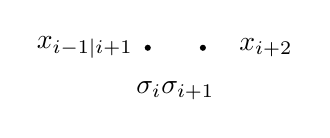
\begin{tikzpicture}[x=1cm,y=1cm]
\node at (0,0) {$x_{\unsure{i-1|i+1}}$};
\fill (0.8,0) circle (1.1pt); \fill (1.5,0) circle (1.1pt);
\node at (2.3,0) {$x_{i+2}$};
\node at (1.15,-.55) {$\sigma_i\sigma_{i+1}$};
\end{tikzpicture}}
\[
\sigma_0\sigma_1,\sigma_1\sigma_2,\ldots,\sigma_{n-2}\sigma_{n-1}
\]
\[
N=\prod_1^{n-1}s_i=\prod_1^{n-1}s'_i=\operatorname{card}G
\qquad G\ni\sigma_0,\ldots,\sigma_{n-1}
\]
\[
\left\{\begin{aligned}
s'_if_{i+1}&=f_is_{i+1}\qquad(0\leq i\leq n-1)\\
s&
\end{aligned}\right.
\qquad
\frac{f_i}{s'_i}=\frac{f_{i+1}}{\unsure{f_{i+1}|s_{i+1}}}=\unsure{f|\delta}
\]

\figure{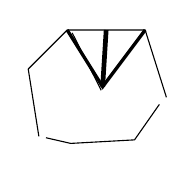
\begin{tikzpicture}[scale=.9]
\draw (0,.65)--(.55,1.2)--(1.65,1.2)--(1.95,.25);
\draw (1.85,.15)--(1.5,-.35)--(.6,-.4)--(.25,-.32);
\draw (.15,-.3)--(0,.65);
\draw[line width=1.2pt] (.55,1.2)--(1.05,.4)--(1.65,1.2);
\draw[line width=1.7pt] (1.05,.4)--(1.1,1.2);
\draw (.62,1.16)--(1.03,.35);
\end{tikzpicture}}

\figure{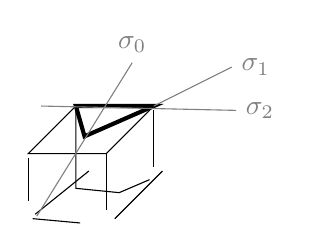
\begin{tikzpicture}[scale=1.1]
\draw (0,1)--(.55,1.55)--(1.45,1.55)--(.9,1)--cycle;
\draw (0,.95)--(0,.45) (.9,1)--(.9,.35) (1.45,1.5)--(1.45,.85);
\draw (.55,1.5)--(.55,.6)--(1.05,.55)--(1.4,.7);
\draw (.05,.25)--(.6,.2) (1,.25)--(1.55,.8);
\draw (.08,.3)--(.7,.8);
\draw[line width=1.5pt] (.55,1.55)--(1.45,1.55)--(.65,1.2)--cycle;
\draw[gray] (.1,.28)--(1.2,2.05) node[above] {$\sigma_0$};
\draw[gray] (1.45,1.55)--(2.35,2) node[right] {$\sigma_1$};
\draw[gray] (.15,1.55)--(2.4,1.5) node[right] {$\sigma_2$};
\end{tikzpicture}}

\figure{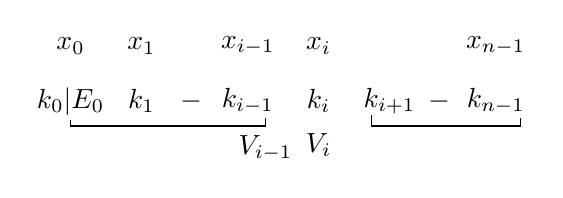
\begin{tikzpicture}[x=.9cm,y=.7cm]
\node at (0,1) {$x_0$}; \node at (1,1) {$x_1$};
\node at (2.5,1) {$x_{i-1}$}; \node at (3.5,1) {$x_i$};
\node at (6,1) {$x_{n-1}$};
\node at (0,0) {$\unsure{k_0|E_0}$}; \node at (1,0) {$k_1$};
\node at (1.7,0) {$-$}; \node at (2.5,0) {$k_{i-1}$};
\node at (3.5,0) {$k_i$}; \node at (4.5,0) {$k_{i+1}$};
\node at (5.2,0) {$-$}; \node at (6,0) {$k_{n-1}$};
\draw (0,-.35)--(0,-.45)--(2.75,-.45)--(2.75,-.3);
\node at (2.75,-.85) {$V_{i-1}$}; \node at (3.5,-.8) {$V_i$};
\draw (4.25,-.25)--(4.25,-.45)--(6.35,-.45)--(6.35,-.3);
\end{tikzpicture}}

\figure{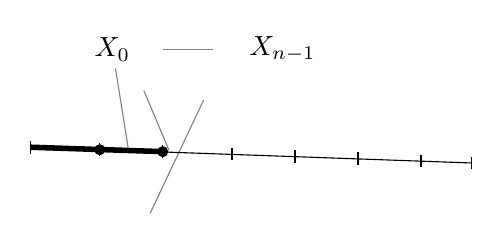
\begin{tikzpicture}[x=.8cm,y=.8cm]
\node at (1.3,1.7) {$X_0$}; \draw[gray] (2.1,1.7)--(2.9,1.7);
\node at (4,1.7) {$X_{n-1}$};
\draw[gray] (1.35,1.4)--(1.55,.15) (1.8,1.05)--(2.2,.1) (2.75,.9)--(1.9,-.9);
\draw (0,.15)--(7,-.1); \draw[line width=2pt] (0,.15)--(2.1,.08);
\foreach \x/\y in {0/.15,1.1/.11,2.1/.08,3.2/.04,4.2/.0,5.2/-.03,6.2/-.07,7/-.1}{\draw (\x,\y+.10)--(\x,\y-.10);}
\fill (1.1,.11) circle (2pt); \fill (2.1,.08) circle (2pt);
\end{tikzpicture}}
% archive sheet number: 123
